\documentclass[12pt,norsk,a4paper,fleqn]{article}
\usepackage[utf8]{inputenc}
\usepackage[norsk]{babel}
% Standard stuff
\usepackage{amsmath,graphicx,varioref,geometry,grffile}
% colors in text
\usepackage[usenames,dvipsnames,svgnames,table]{xcolor}
% Hyper refs
\usepackage[colorlinks]{hyperref}
% Other stuff
\usepackage{float}
\usepackage{placeins} %Keeps figures within given sections
\usepackage{tikz}
\usepackage{CJKutf8}
\usepackage[bottom]{footmisc}   % Place a footnote in an environment in the bottom of the page


% Document formatting
\setlength{\parindent}{0mm}
\setlength{\parskip}{1.5mm}

%Color scheme for listings
\usepackage{textcomp}
\definecolor{listinggray}{gray}{0.9}
\definecolor{lbcolor}{rgb}{0.9,0.9,0.9}

%Listings configuration
\usepackage{listings}
%Hvis du bruker noe annet enn python, endre det her for å få riktig highlighting.
\lstset{
	backgroundcolor=\color{lbcolor},
	tabsize=4,
	rulecolor=,
	language=python,
        basicstyle=\scriptsize,
        upquote=true,
        aboveskip={1.5\baselineskip},
        columns=fixed,
		numbers=left,
        showstringspaces=false,
        extendedchars=true,
        breaklines=true,
        prebreak = \raisebox{0ex}[0ex][0ex]{\ensuremath{\hookleftarrow}},
        frame=single,
        showtabs=false,
        showspaces=false,
        showstringspaces=false,
        identifierstyle=\ttfamily,
        keywordstyle=\color[rgb]{0,0,1},
        commentstyle=\color[rgb]{0.133,0.545,0.133},
        stringstyle=\color[rgb]{0.627,0.126,0.941},
        inputencoding=utf8,
		literate= {æ}{{\ae}}1 {å}{{\aa}}1 {ø}{{\o}}1 {Æ}{{\AE}}1 {Å}{{\AA}}1 {Ø}{{\O}}1
        }
        

\numberwithin{equation}{section}
\newcommand{\blank}[1]{\hspace*{#1}\linebreak[0]}

\usetikzlibrary{shapes,arrows,positioning}


\title{Something something}
\author{Jon André Ottesen}
\date{\today}

\tikzstyle{decision} = [rectangle, draw, fill=red!20, 
    text width=8em, text centered, rounded corners, minimum height=4em]
\tikzstyle{block} = [rectangle, draw, fill=blue!20, 
    text width=8em, text centered, rounded corners, minimum height=4em]
\tikzstyle{line} = [draw, -latex']
\tikzstyle{cloud} = [draw, ellipse,fill=red!20,
    minimum height=2em]
\tikzstyle{start} = [rectangle, draw, fill=green!20, 
text width=8em, text centered, rounded corners, minimum height=4em]

\begin{document}

\begin{flushright}
\small 23.~august, 2019
\end{flushright}
%\title
\textbf{\blank{-10mm}\LARGE Tidsutvikling av utskrevet medisin i Norge}\\
\blank{0mm}FARM3120 – Legemiddelbruk og folkehelse\\
\blank{0mm}{\small Jon André Ottesen}


\section*{Introduksjon}

Denne teksten har som hensikt å lede deg gjennom oppgaven og programmet \textit{farm\_files.py} som skal anvendes i datalabben. Teksten er inndelt i to deler: den første delen omhandler litt generell teori samt informasjon om antiepileptisk medisin som kan knyttes inn i rapporten, og den andre delen fungerer som en dokumentasjon av programmet og dens anvendelse. 


\newpage

\section{Antiepileptika, teori og programmet} \label{sec:01}

\subsection*{Introduksjon}

Programmet som skal anvendes i denne oppgaven ble skrevet med hensikt på antiepileptisk medisin og bruken av dette i befolkningen. Det er derfor meget naturlig at dette står sentralt i oppgaven, men dette betyr \textbf{ikke} at den skal eksklusivt omhandle antiepileptika. Programmet kan anvendes på nesten alle dokumenter fra medisin registeret fra reseptregisteret men mer om dette finnes i seksjon \ref{sec:02}.

\subsection*{Generell teori}

Hopp over

\subsection*{Antiepileptika}

Fertile og gravide kvinner gjennom svangerskapet utgjør populasjonen som undersøkes. En rekke ulike kvalitetsindikatorer benyttes for å se på legemiddelbruk ved ulike indikasjoner og gjennom tidsperioden 2004-2018. Hovedvekt ligger på legemidlet valproat ved epilepsi og bipolar lidelse, som har fått begrensninger for bruk hos fertile kvinner. Basert på aggregerende data vil tidstrender av valproat forskrivning hos fertile kvinner kunne visualiseres.




\newpage


\section{Oppstart} \label{sec:02}

\subsection*{Oppsett og de nødvendige datasett}

Før vi starter å faktisk bruke programmet for å visualisere medikamentbruken i Norge de siste årene kreves det noen steg for at programmet skal fungere.

Disse er:
\begin{enumerate}
\item Datasett fra reseptregisteret\footnote{\url{http://www.reseptregisteret.no/}} om medikamentene som skal undersøkes.

Når det gjelder det første punktet krever programmet at alle filene fra reseptregisteret \textbf{KUN GJELDER FOR ETT LEGEMIDDEL}. Dette betyr at det nødvendig å ha separate filer for f.eks valproat, lamotrigin, antiepileptika (den overordnende kategorien antiepileptika) osv. Når legemiddelet er valgt må \textbf{alt} merkes i kategoriene \textit{Årstall} og \textit{Alder} \textbf{unntatt} ''Alle aldre''. De resterende variabel gruppene \textit{Kjønn} og \textit{Bosted} kan man selv velge hva som skal merkes og være med videre. En bemerkning er at flere merkinger spesielt på kjønn gjør nettsiden lite responsiv. Jeg anbefaler derfor å velge ''Mann'' og ''Kvinne'' og alle stedene under \textit{Bosted} for å unngå mye av dette problemet.

Den siste kategorien er \textit{Måltall}. Som med valget av legemiddel godtar programmet kun at en av valgene er markert. Hovedsaklig er det tenkt at ''Antall brukere'' skal brukes, men hvis det er ønsket å bruke andre typer måletall er det nødvendig å lagre ett nytt datasett der denne variabelen er valgt. Programmet er i all hensikt skrevet med tanke på ''Antall brukere'', og det kan dermed være små feil i teksten visst på plottene men tallene er riktig.

Ett flowchart av prosessen av nedlasting av fra reseptregisteret som kompatibelt med programmet er gitt i figur \ref{fig:flowchart}.

\item Befolkningsdata fra SSB\footnote{\url{https://www.ssb.no/statbank/table/07459/}} eller reseptregisteret, jeg anbefaler reseptregisteret.

Angående punkt to om befolkningsdata anbefaler jeg på det sterkest å bruke de dataene fra reseptregisteret under \textit{Måltall} med navn ''Befolkningsgrunnlag'' istedenfor fra SSB. Ved nedlasting fra reseptregisteret velges de parameterne som datasettet/datasettene du har nedlastet tidligere bruker. Det er her \textbf{NØDVENDIG} å spesifisere et legemiddel men hvilket har ingen betydning\footnote{Grunnen til dette er at programmet leser av spesifikke kolonner i csv-filen og uten et spesifisert legemiddel blir kolonnekombinasjonen forskjøvet en kolonne til venstre. Dette gjør at avlesningen ikke fungerer... Min feil ops.}

\textbf{En veldig viktig kommentar er at datasettet om befolkningen MÅ lagres med navnet 'Befolkning'.}

\item En meget spesifikk lagringsmetode og navnsetting for datasettene fra punkt (1) og (2).

Den siste delen omhandler lagring av datasettene. For at programmet skal kunne lese datasettene er det nødvendig å lagre disse i en eller flere mapper samme sted som programmet er lagret.

For bedre å forstå hvordan datasettene skal lagres skal jeg forklare tankegangen bak lagringen. Som nevnt over må alle datasettene lagres i mapper samme sted som programmet. Poenget med å lagre datasettene i mapper er for å kunne klassifisere legemiddelet etter legemiddeltypen. Tankegangen er nemlig slik at man laster ned ett eller flere datasett om f.eks flere legemidler under klassifikasjonen antiepileptika som valproat og lamotrigin. Denne mappen navngis så etter legemiddeltypen som her ville vært antiepileptika. Videre ville man også lagt inn et datasett om legemiddeltypen med samme navn som mappen. Dette gjør at programmet ser hva som er data for legemiddeltypen og hva som er data for legemiddelet. Endepunktet ville vært mappenavn; Antiepileptika, filnavn; Antiepileptika, Valproat, Lamotrigin osv. Videre skal man da kunne lage en ny mappe om f.eks diabetes eller astma og bruke de som separate tilfeller.

Det er ikke nødvendig med ett datasett navngitt etter legemiddeltypen men uten er det flere funksjoner som ikke vil fungere. Disse er spesifisert nærmere nede i seksjon \ref{sec:03} om anvendelse. Dette betyr at du kan ha en mappe med forskjellige datasett hvor legemiddelene ikke har noe medisinsk korrelasjon, men det er interessant å utregne forskjellige forhold mellom disse eller man kun trenger enkelt plot og grafer.

\end{enumerate}

\textbf{En siste kommentar er at navnet datasettene blir lagret med er navnet du vises med i plottene. Jeg anbefaler dermed på det sterkeste å navngi filene noe meningsfullt som eks navnet på legemiddelet.}


\begin{figure}[H]
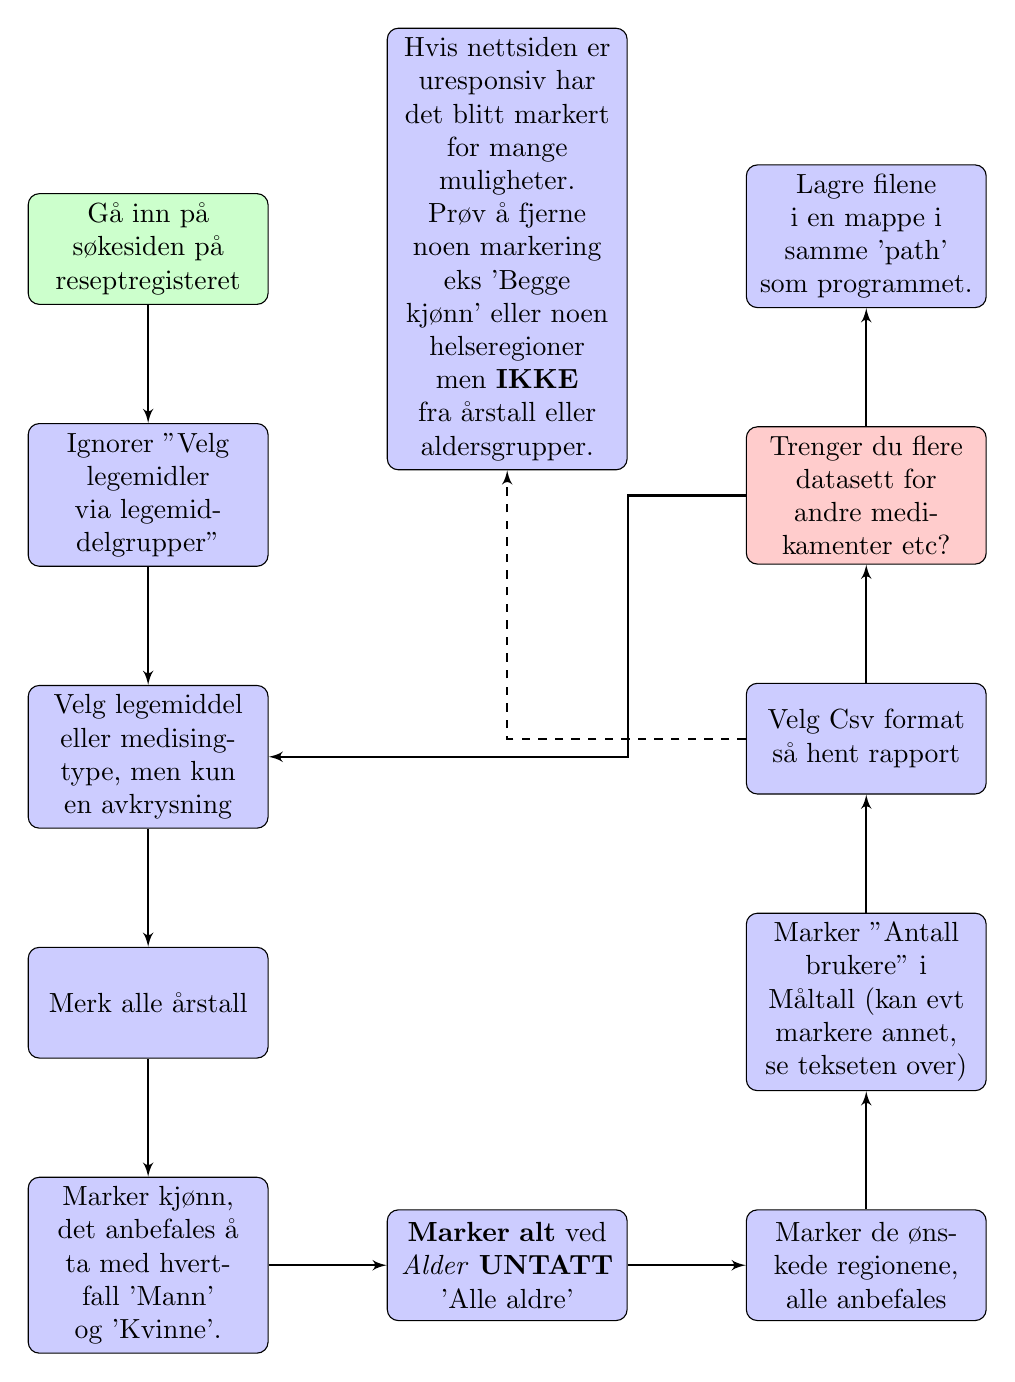
\begin{tikzpicture}[node distance = 15mm, auto]
    % Place nodes
    \node [start] (init) {Gå inn på søkesiden på reseptregisteret};
    \node [block, below = of init] (ignorer) {Ignorer ''Velg legemidler via legemiddelgrupper''};
    \node [block, below = of ignorer] (legemiddel) {Velg legemiddel eller medisingtype, men kun en avkrysning};
    \node[block, below = of legemiddel] (arstall) {Merk alle årstall};
    \node[block, below = of arstall] (kjonn) {Marker kjønn, det anbefales å ta med hvertfall 'Mann' og 'Kvinne'.};
    \node[block, right = of kjonn] (alder) {\textbf{Marker alt} ved \textit{Alder} \textbf{UNTATT} 'Alle aldre'};
    \node[block, right = of alder] (sted) {Marker de ønskede regionene, alle anbefales};
    \node[block, above = of sted] (maltall) {Marker ''Antall brukere'' i Måltall (kan evt markere annet, se tekseten over)};
    \node[block, above = of maltall] (save) {Velg Csv format så hent rapport};
    \node[decision, above = of save] (ferdig) {Trenger du flere datasett for andre medikamenter etc?};
    \node[block, above = of ferdig] (done) {Lagre filene i en mappe i samme 'path' som programmet.};
    \node[block, right = of init] (btw) {Hvis nettsiden er uresponsiv har det blitt markert for mange muligheter. Prøv å fjerne noen markering eks 'Begge kjønn' eller noen helseregioner men \textbf{IKKE} fra årstall eller aldersgrupper.};
    \coordinate[left = of ferdig] (middle);
    \path [line, thick] (init) -- (ignorer);
    \path [line, thick] (ignorer) -- (legemiddel);
    \path [line, thick] (legemiddel) -- (arstall);
    \path [line, thick] (arstall) -- (kjonn);
    \path [line, thick] (kjonn) -- (alder);
    \path [line, thick] (alder) -- (sted);
    \path [line, thick] (sted) -- (maltall);
    \path [line, thick] (maltall) -- (save);
    \path [line, thick] (save) -- (ferdig);
    \path [line, thick] (ferdig) -- (done);
    \path [line, thick] (ferdig) -- (middle) |- (legemiddel);
    \path [line, thick, dashed] (save) -| (btw);
\end{tikzpicture}
	\label{fig:flowchart}
	\caption{Et flowchart om nedlasting av filer fra reseptregisteret.}
\end{figure}

\section*{Anvendelse} \label{sec:03}

Før vi kan stare å anvende programmet er det først nødvendig å åpne Jupyter Notebook. Dette gjøres ved å først åpne kommandovinduet for så å navigere seg frem til mappen med programmet \textit{farm\_files.py}. Dette gjøres med bruk av kommandoen \textit{cd} (change directory) og med 'the path of the folder'\footnote{I mangel på en bra norsk oversettelse.}/miljøet der filen er lagret. Når kommandovinduet er navigert seg til filmappen med programmet skriver man inn 'Jupyter Notebook' og den åpnes. I jupyter notebook lager man så en ny notebook under \textit{new \(\rightarrow\) Python 3}.

Nå som alt er klart kan vi endelig starte å bruke programmet. Det første som \textbf{MÅ} gjøres er å importere de nødvendig pakkene og programmet inn i notebook.
\begin{lstlisting}
from farm_files import visualization as visualization  #Importere programmet for bruk i jupyter
from IPython.display import HTML  #En pakke for å se videoer i jupyter
\end{lstlisting}
Det neste steget er så å initialisere programmet for de forskjellige mappene med datasett.
\begin{lstlisting}
antiep = visualization('Antiepileptika')  #Lage et tilfelle knyttet til mappen Antiepileptika.
respir = visualization('R')  #Ett tilfelle knyttet til mappen om R fra kategorien 'Respirasjonsorganer' på reseptregisteret.
\end{lstlisting}
Datasettene tilknyttet til R er \textbf{KUN} ment for å illustrere hvordan programmet fungerer.

Nå er programmet ferdig initialisert og resten av denne seksjonen vil omhandle kjøreeksempler av programmet. Før dette vil jeg rette oppmerksomheten din til tabell ... hvor alle funksjonen i programmet er listet opp samt argumentene de godtar. Videre i tabell .... er alle variablene listet opp med hvilke input som godtas.

Vi starter med etter min mening den funksjonen {\color{blue}tabell} som bør blir kalt først.
\begin{lstlisting}
antiep.tabell()  #Gir en tabell av variablene for kjønn, legemidler og steder i for Antiepileptika.
respir.tabell()  #Gir en tabell av variablene for kjønn, legemidler og steder i for R.
\end{lstlisting}
Denne er nyttig spesielt siden man kan kopiere variablene og se hvilke variabler som er tilgjengelig. 



\bibliographystyle{plain}
\bibliography{referanser} 

\end{document}
